\documentclass[a4paper, 12pt]{article}
\usepackage[utf8]{inputenc}
\usepackage{palatino}
\usepackage[breaklinks=true]{hyperref}
\usepackage{graphicx}
\usepackage{cprotect}
\usepackage{caption}
\usepackage[left=3cm, right=2cm, top=3cm, bottom=2cm]{geometry}
\geometry{a4paper}
\usepackage{fancyhdr}
\usepackage[brazilian]{babel}
\usepackage{siunitx}
\usepackage{subcaption}
\sisetup{detect-all}
\usepackage{float}
\usepackage{ragged2e}
\pagestyle{fancy}
\renewcommand{\headrulewidth}{0pt} 
\lhead{}\chead{}\rhead{}
\lfoot{}\cfoot{\thepage}\rfoot{}
\graphicspath{{figuras/}}
\usepackage{amsfonts}
\usepackage{mathtools}
\usepackage{cleveref}
\usepackage{spverbatim}
\usepackage[framed,numbered,autolinebreaks,useliterate]{mcode}
\setlength{\parskip}{1em}
\usepackage{xspace}
\usepackage{amsmath}
\usepackage{gensymb}
\usepackage{booktabs}
\usepackage{minted}
\usepackage{listings}
\usepackage{bm}
\usepackage{indentfirst}
\usepackage{algorithm}
\usepackage{algpseudocode, lipsum}
\lstset{
    literate={~} {$\sim$}{1}
}
\usepackage[shortlabels]{enumitem}

\newcommand{\MATLAB}{\textsc{Matlab}\xspace}
\newcommand{\SIMULINK}{\textsc{Simulink}\xspace}
\newcommand{\pspice}{\textsc{PSpice}\xspace}
\newcommand{\Python}{\textsc{Python}\xspace}
\newcommand{\tinkercad}{\textsc{TinkerCad}\xspace}
\newcommand{\arduino}{\textsc{Arduino}\xspace}
\newcommand{\sen}{\hspace{2pt}\mathrm{sen}}
\newcommand{\counts}{\textit{counts}\xspace}
\newcommand{\FT}{\text{F.T.}}
\newcommand{\zeros}{\text{Zeros}}
\newcommand{\polos}{\text{Polos}}
\newcommand{\software}{\textit{software}\xspace}
\newcommand{\hardware}{\textit{hardware}\xspace}
\newcommand{\fitness}{\textit{fitness}\xspace}
\newcommand{\fitsha}{\textit{fitness sharing}\xspace}


\newenvironment{brprocess}[1][]
  {\begin{algorithm}[#1]
     \selectlanguage{brazilian}%
     \floatname{algorithm}{Processo}%
     \renewcommand{\algorithmicif}{\textbf{se}}%
     \renewcommand{\algorithmicfor}{\textbf{para}}%
     \renewcommand{\algorithmicdo}{\textbf{faça}}%
     \renewcommand{\algorithmicthen}{\textbf{faça}}%
     \renewcommand{\algorithmicend}{\textbf{fim}}%
     \renewcommand{\algorithmicwhile}{\textbf{enquanto}}%
     \renewcommand{\algorithmicelse}{\textbf{caso contrário}}%
     % Set other language requirements
  }
  {\end{algorithm}}

  \newenvironment{bralgorithm}[1][]
  {\begin{algorithm}[#1]
     \selectlanguage{brazilian}%
     \floatname{algorithm}{Algoritmo}%
     \renewcommand{\algorithmicif}{\textbf{se}}%
     \renewcommand{\algorithmicfor}{\textbf{para}}%
     \renewcommand{\algorithmicdo}{\textbf{faça}}%
     \renewcommand{\algorithmicthen}{\textbf{faça}}%
     \renewcommand{\algorithmicend}{\textbf{fim}}%
     \renewcommand{\algorithmicwhile}{\textbf{enquanto}}%
     \renewcommand{\algorithmicelse}{\textbf{caso contrário}}%
     % Set other language requirements
  }
  {\end{algorithm}}

\begin{document}
\begin{titlepage}
\newcommand{\HRule}{\rule{\linewidth}{0.5mm}}
	
\centering

\includegraphics[width=0.15\textwidth]{logo-unicamp.pdf}\\[0.5cm]	
\textsc{\Large Universidade Estadual de Campinas}\\[2.0cm]
\textsc{\large Faculdade de Engenharia Elétrica e de Computação}\\[0.5cm]
	
\textsc{IA707/EG507 - Computação Evolutiva}\\[2.5cm]
	
{\LARGE \bfseries EFC II}\\[3.5cm]

\begin{minipage}[t]{0.4\textwidth}
	\begin{flushleft}
    \textit{Alunos}\\
    João Pedro O. Pagnan - 199727
	\end{flushleft}
\end{minipage}
~
\begin{minipage}[t]{0.4\textwidth}
	\begin{flushright}
		\textit{Professor}\\
		Levy Boccato
	\end{flushright}
\end{minipage}\\[4.5cm]

{Campinas, \today}

\vfill\vfill\vfill\vfill\vfill

\includegraphics[width=0.2\textwidth]{logo-feec.png}\\[0.5cm]
\vfill

\end{titlepage}

\justify

Neste exercício, vamos abordar o problema de otimização de função multimodal, com o auxílio de um algoritmo genético (GA, do inglês \textit{genetic algorithm}). Iremos considerar a função contínua
$$f (x, y) = x \cdot \sen(4\pi \cdot x) - y \cdot \sen(4\pi \cdot y + \pi) + 1,$$
onde $x, y \in [-1, 2]$ e desejamos determinar o ponto $(x^{*} , y^{*})$ que maximize a função $f(\cdot )$.
\begin{figure}[H]
    \centering
    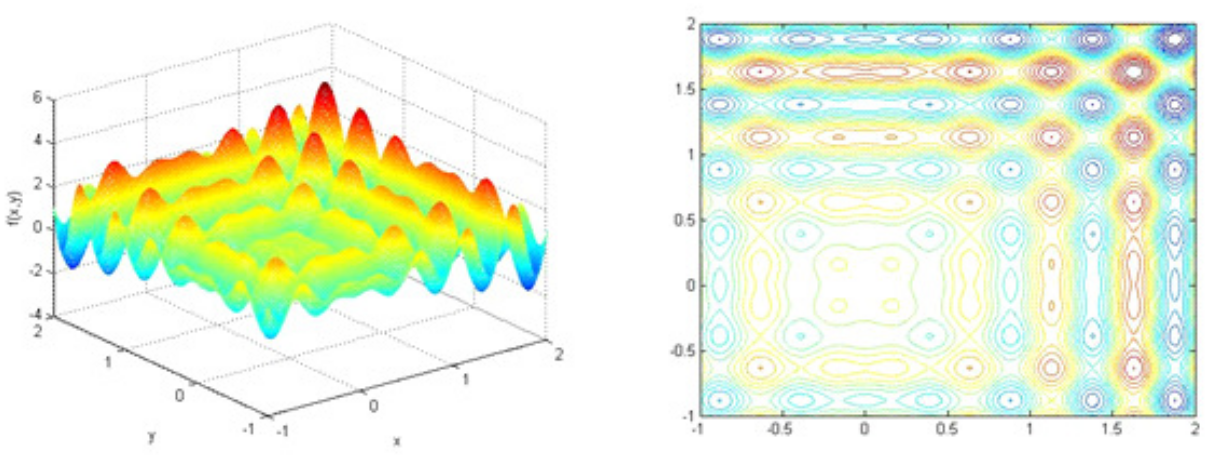
\includegraphics[width=0.8\textwidth]{figuras/grafico-funcao.png}
    \caption{Visualização da superfície e das curvas de nível da função $f (x, y)$.}
    \label{fig:grafico-funcao}
\end{figure}

\textbf{(a) Proponha um algoritmo genético (AG) para encontrar o máximo global de $f(x, y)$. Descreva todos os elementos que o compõem – codificação, função de \fitness, operadores, etc. — e justifique suas escolhas.}

O algoritmo genético para encontrar o máximo global de $f(x, y)$ será composto pelo seguinte passo a passo:
\begin{enumerate}
    \item Gerar a população inicial com $N$ indivíduos representados pela codificação adotada;
    \item Calcular o \fitness para cada indivíduo da população inicial;
    \item Aplicar o operador de seleção para selecionar dois indivíduos baseado em seus \textit{fitness};
    \item Aplicar o operador de recombinação para gerar dois descendentes;
    \item Aplicar o operador de mutação nos descendentes para que os respectivos cromossomos tenham uma probabilidade $p_m$ de serem mutados;
    \item Caso o número total de indivíduos e descendentes for menor que $2N$, repetir do passo 3 ao 5;
    \item Calcular o \fitness dos descendentes;
    \item Eliminar os $N$ indivíduos de menor \fitness;
    \item Repetir do passo 3 ao 8 até o critério de parada ser atingido.
\end{enumerate}

No caso, a codificação adotada escolhida foi a \textbf{codificação real}, em que cada indivíduo, ou solução, é representada por um vetor bidimensional cujos elementos são números reais, isto é, sendo $\bm{z}$ um indivíduo da população:
\begin{equation}
    \bm{z} = \left[x, y \right],
\end{equation}
com $x,y \in [-1, 2]$.

A \textbf{geração da população inicial} será da forma indicada no processo \ref{alg:pop-inicial}, sendo $N$ o tamanho da população.
\begin{brprocess}[!ht]
    \textbf{Paramêtros}: Tamanho da população desejada\\
    \textbf{Saída}: População gerada
    \cprotect\caption{Geração aleatória da população inicial (\verb|gerar_pop(N)|)}
    \begin{algorithmic}
    \State população $\gets [\;]$
    \State $i\gets 0$
    \While{$i < N$}
        \State cromossomo $\gets [\;]$
        \State $j \gets 0$
        \While{$j < 2$}
            \State gene $\gets$ alelo $\in [-1, 2]]$
            \State cromossomo $[j] \gets$ gene
            \State $j \gets j + 1$
        \EndWhile
        \State \textit{fitness} $\gets 0$
        \State população $[i] \gets$ [cromossomo, \textit{fitness}]
        \State $i \gets i + 1$
    \EndWhile
    \State \textbf{retorna} população
    \end{algorithmic}
    \label{alg:pop-inicial}
\end{brprocess}

No caso, o primeiro alelo do cromossomo se refere à variável $x$ e o segundo à variável $y$.

\textbf{Observação:} Como o algoritmo genético será implementado em \Python, foi considerado que a coordenadas dos elementos dos vetores se iniciam em 0.

Na segunda etapa do algoritmo genético tem-se o \textbf{cálculo do valor da função de avaliação}. No caso, a função de avaliação, ou \fitness, adotada é a própria função que deseja-se maximizar. Dessa forma, o cálculo é dado por:
\begin{equation}\label{eq:fitness}
    \phi(\bm{z}) = \phi(x, y) = x \cdot \sen(4\pi \cdot x) - y \cdot \sen(4\pi \cdot y + \pi) + 1
\end{equation}

Com isso, o processo que define o cálculo do \fitness é descrito da forma indicada no processo \ref{alg:fitness}.
\begin{brprocess}[!ht]
\textbf{Entradas}: população\\
\textbf{Saída}: população com os valores de \fitness atualizado
\cprotect\caption{Cálculo do \fitness (\verb|calc_fitness(populacao)|)}
\begin{algorithmic}
\For{indivíduo \textbf{em} população}
    \If{indivíduo[1] = 0}
        \State{$x =$ indivíduo$[0][0]$}
        \State{$y =$ indivíduo$[0][1]$}
        \State{\fitness = $x \cdot \sen(4\pi \cdot x) - y \cdot \sen(4\pi \cdot y + \pi) + 1$}
        \State indivíduo[1] = \fitness
    \EndIf
\EndFor
\State \textbf{retorna} população
\end{algorithmic}
\label{alg:fitness}
\end{brprocess}

Na terceira etapa, o GA aplica o \textbf{operador de seleção por torneio} na população. Esse método utiliza o parâmetro $q$, que é igual à quantidade de indivíduos da população selecionados por torneio. Esse método é executado duas vezes no algoritmo genético, de forma a determinar dois pais para a recombinação e é descrito pelo processo \ref{alg:selecao}.
\begin{brprocess}[!ht]
    \cprotect\caption{Operador de seleção por torneio (\verb|selecao_torneio(populacao,|
    \verb|N, q_torneio)|}
    \textbf{Entrada:} população\\
    \textbf{Parâmetros}: quantidade de indivíduos da população selecionados por torneio e tamanho da população inicial\\
    \textbf{Saída}: o melhor indivíduo escolhido no torneio
    \begin{algorithmic}
            \State $i \gets 0$
            \State indivíduos participantes $\gets [\;]$
            \While{$i < q$}
                \State índice indivíduo selecionado $\gets n \in \{0, 1, ..., N - 1\}$
                \State indivíduos participantes $[i] \gets$ população [índice indivíduo selecionado]
                \State $i \gets i + 1$
            \EndWhile
            \State índice do melhor indivíduo $\gets$ indivíduos participantes[\verb|argmax|(indivíduos participantes [:,1]])
            \State melhor indivíduo $\gets$ indivíduos participantes[índice do melhor indivíduo]
            \State \textbf{retorna} melhor indivíduo
    \end{algorithmic}
    \label{alg:selecao}
\end{brprocess}

Este operador foi escolhido por possibilitar o ajuste da pressão seletiva na população através do parâmetro $q$.

Em seguida, na quarta etapa, o \textbf{operador de recombinação} escolhido foi o método de \textit{crossover} aritmético. Nele, os filhos gerados resultam de uma combinação linear dois pais. Esse método foi escolhido por ser bem apropriado para problemas de otimização numérica com restrições onde a região factível é convexa. Esse é o caso para o problema que deseja-se resolver.

Sendo $P1$ e $P2$ os pais e $D1$ e $D2$ os descendentes, esse método é descrito pelo processo \ref{alg:recombinacao}.
\begin{brprocess}[!ht]
    \cprotect\caption{Operador de recombinação (\verb|crossover_aritmetico(cromossomo_p1,|
    \verb|cromossomo_p2,| \verb|min,| \verb|max|)}
    \textbf{Entrada}: cromossomo dos dois pais, mínimo e máximo do espaço de busca\\
    \textbf{Saída}: cromossomo de ambos os filhos
    \begin{algorithmic}
        \State $i \gets 0$
        \State descendentes $\gets [\;]$
        \State $a \gets \text{número aleatório} \in [0, 1]$
        \While{$i < 2$}
            \If{$i = 0$}
                \State \text{filho}$_1 \gets a \cdot \text{pai}_1 + (1 - a) \cdot \text{pai}_2$
                \State $i \gets i + 1$
            \EndIf
            \If{$i = 1$}
                \State \text{filho}$_1 \gets (1 - a) \cdot \text{pai}_1 + a \cdot \text{pai}_2$
                \State $i \gets i + 1$
            \EndIf
        \EndWhile
        \State \textbf{retorna} descendentes
    \end{algorithmic}
    \label{alg:recombinacao}
\end{brprocess}

Por fim, resta detalhar o \textbf{operador de mutação} utilizado. Neste caso, foi escolhido a \textbf{mutação uniforme}, que consiste em pegar uma fração do intervalo de busca, que chamaremos de $f_m$, e, a partir disso, será determinado o intervalo da distribuição $r = f_m \cdot (max-min)$, de forma que a distribuição uniforme é dada por $U(-r,r)^l$.

O processo pode ser descrito da forma indicada no processo \ref{alg:mutacao}.
\begin{brprocess}[!ht]
    \cprotect\caption{Operador de mutação (\verb|mutacao_uniforme(cromossomo,|
    \verb|p_mutacao,|\verb|f_mutacao,| \verb|min,| \verb|max|)}
    \textbf{Entrada}: cromossomo a ser mutado e valores mínimo e máximo do espaço de busca\\
    \textbf{Parâmetros}: probabilidade da mutação ocorrer e fator de mutação que vai determinar um intervalo em que o gene pode ser mutado\\
    \textbf{Saída}: cromossomo mutado
    \begin{algorithmic}
        \State $i \gets 0$
        \State{número $\gets k \in \{0, ..., p_m\, ..., 1\}, k \in \mathbb{R}$}
        \For{i \textbf{em} len(cromossomo)}
            \If{indivíduo[1] = 0}
                \State{range-mutacao $\gets (max - min)\cdot f_m$}
                \State {valor-mutacao $\gets r \in \{$-range-mutacao, range-mutacao$\}, r \in \mathbb{R}$}
                \State {cromossomo[i] $\gets$ cromossomo[i] + valor-mutacao}
                \If{cromossomo[i]$<$ min}
                    \State {cromossomo[i] $\gets$ min}
                \EndIf
                \If{cromossomo[i]$>$ max}
                    \State {cromossomo[i] $\gets$ max}
                \EndIf
            \EndIf
        \EndFor
    \end{algorithmic}
    \label{alg:mutacao}
\end{brprocess}

\textbf{(b) Para cada uma de 5 execuções independentes do AG, apresente as curvas de \fitness médio e de \fitness do melhor indivíduo em função do número de gerações. Mostre também, tendo por pano de fundo as curvas de nível da função $f(x, y)$, a distribuição dos indivíduos da população final em cada execução. Com base nesse conjunto de gráficos, busque analisar o algoritmo em termos de sua eficiência de busca e manutenção de diversidade.}

\textbf{(c) Implemente agora o método de \fitsha. Comente as escolhas feitas para os valores dos parâmetros (e.g., $\sigma_s$) e de operadores (caso alguma modificação em relação ao item (b) tenha sido necessária). Repita o procedimento do item (b) para analisar o comportamento do \fitsha.}

\textbf{(d) Introduza, por fim, o esquema de restrição de cruzamento (seguindo o espírito da abordagem de especiação) proposto por \cite{deb1989genetic} Analise o impacto da inserção deste mecanismo na evolução da população e, em última análise, no desempenho do algoritmo.}

\clearpage

\bibliographystyle{ieeetr}

\bibliography{bib}

\pdfinfo{
   /Title  (IA707 - EFC II - 199727)
}
 \end{document}